
\documentclass[a4paper, anonymous, numberwithinsect, pdfa, UKenglish,cleveref, autoref, thm-restate]{socg-lipics-v2021}

\usepackage{algorithmicx}
\usepackage{algorithm}
\usepackage[noend]{algpseudocode}

\usepackage{tikz}
\usetikzlibrary{shapes.geometric}
\usetikzlibrary{arrows.meta}
\usepackage{indentfirst}
%This is a template for producing LIPIcs articles. 
%See lipics-v2021-authors-guidelines.pdf for further information.
%for A4 paper format use option "a4paper", for US-letter use option "letterpaper"
%for british hyphenation rules use option "UKenglish", for american hyphenation rules use option "USenglish"
%for section-numbered lemmas etc., use "numberwithinsect"
%for enabling cleveref support, use "cleveref"
%for enabling autoref support, use "autoref"
%for anonymousing the authors (e.g. for double-blind review), add "anonymous"
%for enabling thm-restate support, use "thm-restate"
%for enabling a two-column layout for the author/affilation part (only applicable for > 6 authors), use "authorcolumns"
%for producing a PDF according the PDF/A standard, add "pdfa"

\pdfoutput=1 %uncomment to ensure pdflatex processing (mandatatory e.g. to submit to arXiv)
%\hideLIPIcs  %uncomment to remove references to LIPIcs series (logo, DOI, ...), e.g. when preparing a pre-final version to be uploaded to arXiv or another public repository

%\graphicspath{{./graphics/}}%helpful if your graphic files are in another directory
\newcommand{\br}[1]{\left( #1 \right)}
\newcommand{\brc}[1]{\left\{ #1 \right\}}
\newcommand{\spr}[1]{\left| #1 \right|}
\newcommand{\fl}[1]{\left\lfloor #1 \right\rfloor}
\newcommand{\cl}[1]{\left\lceil #1 \right\rceil}
\newcommand{\angl}[1]{\langle #1 \rangle}
\newcommand{\e}[1]{\exp\left\{ #1 \right\}}
\newcommand{\diam}{\operatorname{diam}}
\newcommand{\NPcomplete}{\textnormal{$\mathcal{NP}$-Complete}}
\newcommand{\NPhard}{\textnormal{$\mathcal{NP}$-Hard}}
\newcommand{\polyAPXcomplete}{\textnormal{Poly-$\mathcal{APX}$-Complete}}
\newcommand{\Cent}{\texttt{Cent}}
\newcommand{\APP}{\texttt{APP}}
\newcommand{\OPT}{\texttt{OPT}}
\newcommand{\COST}{\texttt{COST}}
\newcommand{\argmin}{\operatorname*{arg\,min}}
\newcommand{\argmax}{\operatorname*{arg\,max}}


\bibliographystyle{plainurl}% the mandatory bibstyle

\title{Searching in trees with heavy group sets of fixed size} %TODO Please add

\titlerunning{Searching in trees with heavy group sets of fixed size} %TODO optional, please use if title is longer than one line

\author{Michał {Szyfelbein}}{Faculty of Electronics, Telecommunications and Informatics, Gdańsk University of Technology, Poland \and  }{s193307@student.pg.edu.pl}{https://orcid.org/0009-0009-9894-9671}{}%TODO mandatory, please use full name; only 1 author per \author macro; first two parameters are mandatory, other parameters can be empty. Please provide at least the name of the affiliation and the country. The full address is optional. Use additional curly braces to indicate the correct name splitting when the last name consists of multiple name parts.


\authorrunning{M. Szyfelbein} %TODO mandatory. First: Use abbreviated first/middle names. Second (only in severe cases): Use first author plus 'et al.'

\Copyright{Michał Szyfelbein} %TODO mandatory, please use full first names. LIPIcs license is "CC-BY";  http://creativecommons.org/licenses/by/3.0/

\begin{CCSXML}
<ccs2012>
   <concept>
       <concept_id>10003752.10003777.10003782</concept_id>
       <concept_desc>Theory of computation~Oracles and decision trees</concept_desc>
       <concept_significance>500</concept_significance>
       </concept>
   <concept>
       <concept_id>10003752.10003809.10003635</concept_id>
       <concept_desc>Theory of computation~Graph algorithms analysis</concept_desc>
       <concept_significance>500</concept_significance>
       </concept>
   <concept>
       <concept_id>10003752.10003809.10003636</concept_id>
       <concept_desc>Theory of computation~Approximation algorithms analysis</concept_desc>
       <concept_significance>500</concept_significance>
       </concept>
   <concept>
       <concept_id>10003752.10003809.10010052.10010053</concept_id>
       <concept_desc>Theory of computation~Fixed parameter tractability</concept_desc>
       <concept_significance>500</concept_significance>
       </concept>
   <concept>
       <concept_id>10003752.10003809.10011254.10011257</concept_id>
       <concept_desc>Theory of computation~Divide and conquer</concept_desc>
       <concept_significance>500</concept_significance>
       </concept>
 </ccs2012>
\end{CCSXML}

\ccsdesc[500]{Theory of computation~Oracles and decision trees}
\ccsdesc[500]{Theory of computation~Graph algorithms analysis}
\ccsdesc[500]{Theory of computation~Approximation algorithms analysis}
\ccsdesc[500]{Theory of computation~Fixed parameter tractability}
\ccsdesc[500]{Theory of computation~Divide and conquer}
%TODO mandatory: Please choose ACM 2012 classifications from https://dl.acm.org/ccs/ccs_flat.cfm 

\keywords{Graph Searching, Binary Search, Decision Trees, Vertex Ranking, Graph Theory, Approximation Algorithm, Parametrized complexity, Trees} %TODO mandatory; please add comma-separated list of keywords

\category{} %optional, e.g. invited paper

\relatedversion{} %optional, e.g. full version hosted on arXiv, HAL, or other respository/website
%\relatedversiondetails[linktext={opt. text shown instead of the URL}, cite=DBLP:books/mk/GrayR93]{Classification (e.g. Full Version, Extended Version, Previous Version}{URL to related version} %linktext and cite are optional

%\supplement{}%optional, e.g. related research data, source code, ... hosted on a repository like zenodo, figshare, GitHub, ...
%\supplementdetails[linktext={opt. text shown instead of the URL}, cite=DBLP:books/mk/GrayR93, subcategory={Description, Subcategory}, swhid={Software Heritage Identifier}]{General Classification (e.g. Software, Dataset, Model, ...)}{URL to related version} %linktext, cite, and subcategory are optional

%\funding{(Optional) general funding statement \dots}%optional, to capture a funding statement, which applies to all authors. Please enter author specific funding statements as fifth argument of the \author macro.

\acknowledgements{The author wants to thank Dariusz Dereniowski for the preliminary discussions and guidance}%optional

%\nolinenumbers %uncomment to disable line numbering



%Editor-only macros:: begin (do not touch as author)%%%%%%%%%%%%%%%%%%%%%%%%%%%%%%%%%%
\EventEditors{John Q. Open and Joan R. Access}
\EventNoEds{2}
\EventLongTitle{42nd Conference on Very Important Topics (CVIT 2016)}
\EventShortTitle{CVIT 2016}
\EventAcronym{CVIT}
\EventYear{2016}
\EventDate{December 24--27, 2016}
\EventLocation{Little Whinging, United Kingdom}
\EventLogo{}
\SeriesVolume{42}
\ArticleNo{23}
%%%%%%%%%%%%%%%%%%%%%%%%%%%%%%%%%%%%%%%%%%%%%%%%%%%%%%

\begin{document}

\maketitle

%TODO mandatory: add short abstract of the document
\begin{abstract}

We consider the following generalization of the binary search problem: A searcher is required to find a hidden element $x$ in a tree $T$. To do so, they iteratively perform queries to an oracle about a chosen vertex $v$. After each such call, the oracle responds whether the target was found and if not, the searcher receives as a reply the neighbor of $v$ that lays on the shortest path towards $x$. Additionally, each vertex $v$ may have a different query cost $w(v)$. The goal is to find the optimal querying strategy for the searcher which minimizes the worst case query cost required to find $x$. The problem is known to be NP-hard even in restricted classes of trees such as bounded diameter spiders [Cicalese et al. 2016] and no constant factor approximation algorithm is known for the general case. Inspired by recent studies [Dereniowski et al. 2022, Dereniowski et al. 2024], instead of restricted classes of trees, we explore restrictions on the weight function. We introduce the concept of a heavy group set of a vertex $HG(v,w)$. We show that if for every $v\in T$: $|HG\br{v,w}|\leq k$ an $O(\log\log n)$-approximation can be found within $2^{O(\log^2k)}\cdot\text{poly}(n)$ time.  
\end{abstract}

\section{Introduction}
Searching plays a pivotal role in computer science, serving as a cornerstone for numerous theoretical models and real-world applications. Many computational problems, such as sorting, can be framed as searching for an element within a well-defined set or rely on searching as a fundamental subroutine. The significance of efficient search strategies spans multiple domains, including data management systems, artificial intelligence, and operations research.

One of the most well-known search models is the classical binary search, which efficiently locates a given value within a linearly ordered set. A common application of binary search arises in experimental measurements, where each comparison corresponds to performing a measurement to determine whether the target value is smaller or greater than a chosen threshold. This problem can be formulated as searching within a path, where each comparison operation is modeled as a query to an oracle. In constant time, the oracle returns information on whether a given vertex is the target and, if not, which subpath of the original path contains it.

\subsection{Problem description}
\begin{figure}[htbp]
    \begin{minipage}[t]{0.47\textwidth}
        \centering
        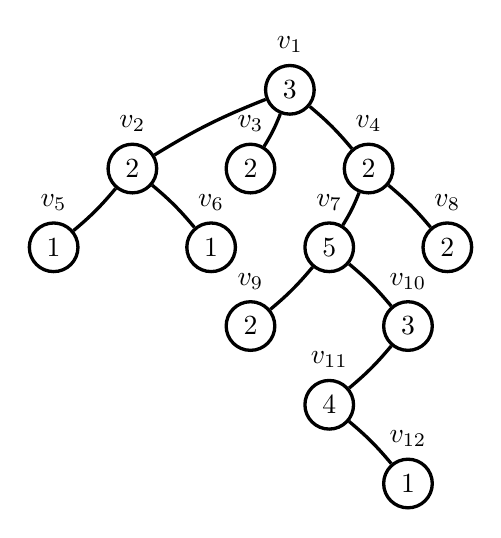
\begin{tikzpicture}[every node/.style={draw, very thick}, every path/.style={very thick}]
        
        \node[circle, draw, label=above:{$v_1$}] (1) at (-1,10) {3};
        \node[circle, draw, label=above:{$v_2$}] (2) at (-3,9) {2};
        \node[circle, draw, label=above:{$v_3$}] (3) at (-1.5,9) {2};
        \node[circle, draw, label=above:{$v_4$}] (4) at (0,9) {2};
        \node[circle, draw, label=above:{$v_5$}] (5) at (-4,8) {1};
        \node[circle, draw, label=above:{$v_6$}] (6) at (-2,8) {1};
        \node[circle, draw, label=above:{$v_7$}] (7) at (-0.5,8) {5};
        \node[circle, draw, label=above:{$v_8$}] (8) at (1,8) {2};
        \node[circle, draw, label=above:{$v_9$}] (9) at (-1.5,7) {2};
        \node[circle, draw, label=above:{$v_{10}$}] (10) at (0.5,7) {3};
        \node[circle, draw, label=above:{$v_{11}$}] (11) at (-0.5,6) {4};
        \node[circle, draw, label=above:{$v_{12}$}] (12) at (0.5,5) {1};
        
        \draw[bend right=5] (1) to (2);
        \draw[bend left=5] (1) to (3);
        \draw[bend left=5] (1) to (4);
        \draw[bend left=5] (2) to (5);
        \draw[bend left=5] (2) to (6);
        \draw[bend left=5] (4) to (7);
        \draw[bend left=5] (4) to (8);
        \draw[bend left=5] (7) to (9);
        \draw[bend left=5] (7) to (10);
        \draw[bend left=5] (10) to (11);
        \draw[bend left=5] (11) to (12);
        
        \end{tikzpicture}
        \caption{A tree $T$ with $k\br{T}=5$. For example: $HG(v_4)=\brc{\brc{v_1},\brc{v_7,v_{10},v_{11}}}$ and $HG(v_{10})=\brc{\brc{v_7},\brc{v_{11}}}$.}\label{exampleInputTree}
    \end{minipage}%
    \hspace{0.06\textwidth} % Add space between the two minipages
    \begin{minipage}[t]{0.47\textwidth}
        \centering
        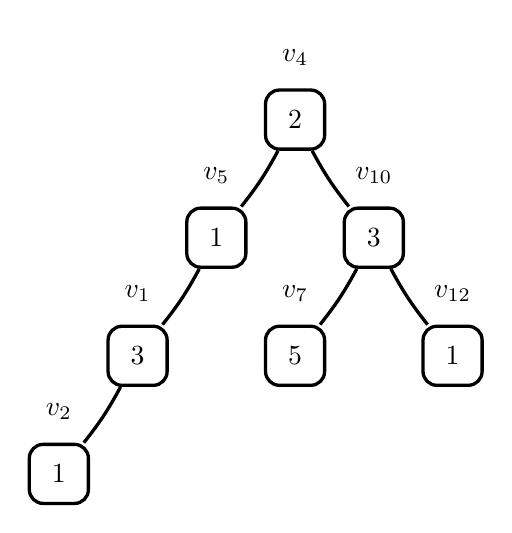
\begin{tikzpicture}[every node/.style={draw, minimum size=0.75cm, rounded corners=5pt, very thick}, every path/.style={very thick}]
        
        \node[rectangle, draw, label=above:{$v_4$}] (1) at (0,10) {2};
        \node[rectangle, draw, label=above:{$v_5$}] (2) at (-1,8.5) {1};
        \node[rectangle, draw, label=above:{$v_{10}$}] (3) at (1,8.5) {3};
        \node[rectangle, draw, label=above:{$v_1$}] (4) at (-2,7) {3};
        \node[rectangle, draw, label=above:{$v_7$}] (5) at (0,7) {5};
        \node[rectangle, draw, label=above:{$v_{12}$}] (6) at (2,7) {1};
        \node[rectangle, draw, label=above:{$v_2$}] (7) at (-3,5.5) {1};
        
        \draw[bend left=5] (1) to (2);
        \draw[bend right=5] (1) to (3);
        \draw[bend left=5] (2) to (4);
        \draw[bend left=5] (3) to (5);
        \draw[bend right=5] (3) to (6);
        \draw[bend left=5] (4) to (7);
        
        \end{tikzpicture}
        \caption{A decision tree $D$ for $T$ of cost $10$. Notice that queries to $v_3, v_6, v_8,v_9$ and $v_{11}$ were omitted}\label{exampleDecisionTree}
    \end{minipage}
\end{figure}
In this work, we explore a generalization of the problem by extending it to tree structures with non-uniform query costs. Specifically, we consider a vertex-weighted tree 
$T$, where the weight $w$ of a vertex represents the time required to query it (for example see Figure \ref{exampleInputTree}). The search strategy, modeled as a decision tree $D$ (for example see Figure \ref{exampleDecisionTree}), aims to locate a hidden target vertex 
$x$ by querying vertices of the input tree 
$T$. A query to vertex 
$v$ after $w\br{v}$ units of time provides one of the two types of responses: either confirming that 
$v$ is the target vertex, thus terminating the search, or revealing the neighbor of $v$ laying on the shortest path towards $x$. The quality of the decision tree is measured by its depth, i. e. the worst-case search time for an arbitrary vertex in $T$. 

The problem is known to be NP-hard in several classes of trees \cite{DereniowskiVxRankOfChGsAndWTs, Dereniowski2009ERankOfWTs,Cicalese2012BinIdentPForWTs,Cicalese2016OnTSPwNonUniCost}. Furthermore, no constant-factor approximation algorithm is currently known, and the state-of-the-art approach achieves an  $O\br{\sqrt{\log n}}$ approximation \cite{dereniowski2017ApproxSsForGeneralBSinWTs} for general trees. In recent years, constant-factor approximation algorithms have been developed for restricted weight functions \cite{dereniowski2022CFApproxAlgForBSInTsWithMonoQTimes, dereniowski2024SInTsMonoQTs}. Inspired by this progress, we introduce a novel approach for a different restriction on the weight function, specifically for trees with heavy group sets of fixed size.

Let $v\in V$. We define a \textit{heavy group} with respect to $v$ as $H\subseteq V\br{T}$ such that: $T[H]$ is connected, for every $u \in H$: $w\br{u}>w\br{v}$ and $H$ is maximal - no vertex can be added to it without violating one of its properties. We then define the \textit{heavy group set} of $v$ as: $HG\br{v,w}=\brc{H|H \text{ is a heavy group w. r. t. } v}$. We define the \textit{heavy group sets size} of $T$ as $k\br{T, w}=\max_{v\in V\br{T}}\brc{\spr{HG\br{v,w}}}$. Whenever clear from the context we will write $k\br{T}$ or just $k$.

We study the problem under the assumption that $k$ is fixed.
The motivation behind such restriction is drawn from the fact that the hardness of the problem (and its approximation) occurs due to alternating groups of vertices with high and low weights. However, when this does not happen too often the problem can be approximated efficiently.
\subsection{State-of-the-art and related results}
One can distinguish several research directions related to our problem. Below the main results for each model are listed separately:

\paragraph*{Vertex Query Model in Trees}
For unweighted trees, the optimal search strategy can be computed in linear time, as shown independently in \cite{OnakParys2006GenOfBSSInTsAndFLikePosets} and \cite{Schaffer1989OptNodeRankOfTsInLinTime}. The weighted version, however, becomes strongly NP-hard and is FPT (fixed-parameter tractable) with respect to the maximum weight among vertices \cite{DereniowskiVxRankOfChGsAndWTs}. Weighted paths admit a dynamic programming solution with $O(n^2)$ running time \cite{Cicalese2012BinIdentPForWTs, LaberOnBSWithNonUniCosts}. For general trees, a polynomial-time $O(\sqrt{\log n})$-approximation exists \cite{dereniowski2017ApproxSsForGeneralBSinWTs}, derived from a QPTAS achieving $(1+\varepsilon)$-approximation in $n^{O(\log n / \varepsilon^2)}$ time. Related versions of the problem include change of criterion to the average case both in weighted \cite{Cicalese2016DecTreesSimEval, Dasgupta} and unweighted setups \cite{SplayTonT, Fast_app_centroid_trees}. Note, that in this version of the problem the weight is usually called cost, and sometimes a function called probability/weight is introduced which denotes how often each vertex is searched for.

\paragraph*{Edge Query Model in Trees}
Unweighted edge search in trees requires intricate algorithms despite linear running time \cite{Lam1998ERankOfGsIsH, Mozes_Onak2008FindOptTSStartInLinTime}. Upper bounds on depths of the strategy are discussed in \cite{LaberFastSInTs, MAKINOOnMinERankSTs, DereniowskiEfPQProcByGRank, Emamjomeh2016DetAndProbBSinGs}. The weighted edge search is NP-hard even for restricted tree classes: trees of degree $\Delta\br{T}\geq 3$ \cite{Cicalese2012BinIdentPForWTs} and spiders of diameter $\diam\br{T}\geq6$ \cite{Cicalese2016OnTSPwNonUniCost}. Paths and trees with diameter $\diam\br{T}\leq5$ allow polynomial-time solutions \cite{Cicalese2012BinIdentPForWTs}. Approximation ratios range from $O(\log n)$ in \cite{Dereniowski2009ERankOfWTs}, to slightly improved $O(\log n / \log \log \log n)$ in \cite{Cicalese2012BinIdentPForWTs} and  $O(\log n / \log \log n)$ in \cite{Cicalese2016OnTSPwNonUniCost}. For the average case weighted \cite{Cicalese2016DecTreesSimEval, Dasgupta} and unweighted setups \cite{Jacobs2010OnTheComplexSearchInTsAvg,Cicalese2014ImprovedApproxAvgTs, Hgemo2024TightAB} are considered. 

\paragraph*{Searching in Posets}
Searching in partially orderer sets with uniform query times is NP-hard even for bounded-height Hasse diagrams \cite{CarmoSInRandPOSets, DereniowskiERAndSInPOSets}. Randomized approaches and branchings yield an $O(\log n / \log \log n)$-approximation for posets with maximum elements \cite{DereniowskiERAndSInPOSets}. Posets with minimum elements admit linear-time algorithms with additive error 1 \cite{OnakParys2006GenOfBSSInTsAndFLikePosets}. The equivalence between edge ranking and tree-like poset searching is highlighted in \cite{DereniowskiERAndSInPOSets}.

\subsection{Organization of the paper}
In Section \ref{preliminaries}, we provide the necessary formal definitions required for the analysis (Sections \ref{notationAndQueryModel} and \ref{definitionOfDecisionTree}).

In Section \ref{parametrizedSolution}, we present the main result of the paper, namely the $O\br{\log\log n}$-approximate algorithm running in $2^{O\br{\log^2k}}\cdot\text{poly}\br{n}$ time. To achieve this, we introduce the concept of weight levels and the notion of contracting heavy child groups in Section \ref{wLvlsAndGrpContraction}. We also invoke the definition of the vertex ranking in Section \ref{vertexRanking}. In Section \ref{mainRecursiveProcedure}, this allows us to construct a recursive procedure that firstly contracts all heavy groups belonging to the highest weight level, then recursively builds the solution for this modified tree and at last expands the contracted groups to extend the solution to the entire tree (the formal analysis of the latter is deferred to Section \ref{extendingTheDecisionTree}).

In Section \ref{extendingTheDecisionTree}, we present an algorithm which extends the solution for the contracted tree to all vertices of the input tree without introducing excessive error. This is done by building an auxiliary tree $T_{\mathcal{Z}}$ from subset of $V\br{T}$, then creating a new decision tree for $T_{\mathcal{Z}}$ and at last, merging this strategy with the previous solution.
\section{Preliminaries}\label{preliminaries}
\subsection{Notation and query model}\label{notationAndQueryModel}

The \textit{Tree Search Problem} consists of a triple $T=\br{V\br{T},E\br{T},w}$, where $w:V\br{T}\to \mathbb{R}_{+}$ is the cost of querying each vertex. A \textit{query} to an oracle asks about chosen vertex and after time $w(v)$ receives an answer. If the answer is affirmative, then $v$ is the target, otherwise a neighbor $u$ of $v$ is returned such $u$ belongs to the path between $v$ and $x$. 

We assume that each considered tree $T$ is rooted at some vertex $r\br{T}$ and additionally, we assume that every input tree is rooted at $\argmin_{v\in V\br{T}}\brc{w\br{v}}$. Ties are broken arbitrarily. By $uv\in E\br{T}
$ we denote an edge connecting vertices $u$ and $v$. For any $V'\subseteq V\br{T}$ by $T[V']$ we denote the forest, being the subgraph of $T$ induced by $V'$. Additionally, by $T\angl{V'}$ we denote the minimal connected subtree of $T$ containing all vertices from $V'$. We denote the set of neighbors of $v\in V\br{T}$ as $N_T\br{v} = \brc{u\in V\br{T}|uv\in E\br{T}}$. We denote the set of neighbors of subtree $T'$ of $T$ as $N_T\br{T'} = \bigcup_{v\in V\br{T'}}N_T\br{v}-V\br{T'}$. By $\deg_{T}\br{v}=\spr{N_T\br{v}}$ we denote the degree of $v$ in $T$. By $\mathcal{P}_{T}\br{u, v}=T\angl{\brc{u,v}}-\brc{u,v}$ we denote a path of vertices between $u$ and $v$ in $T$ (excluding $u$ and $v$). Analogously for $V_1,V_2\in V\br{T}$ we define $\mathcal{P}_{T}\br{V_1, V_2}=T\angl{V_1\cup V_2}-\br{V_1\cup V_2}$.
% For a set $U\subseteq V$ and a target $x\in T$ by $T\angl{U,x}$ we will denote the maximal subtree of $T-U$ such that $x\in T\angl{U,x}$.

\subsection{Definition of a decision tree}\label{definitionOfDecisionTree}
\begin{definition}
A decision tree is triple $D=(V\br{D}, E\br{D}, m)$ where $V\br{D}$ are vertices and $E\br{D}$ are edges of $D$ and $m: V\br{D} \to V\br{T}$. Let $Q_D\br{T,x}$ be the sequence of queries performed in order to find $x$ using decision tree $D$ in $T$. We define the cost of searching for target $x$ using decision tree $D$ in $T$ with weight function $w$ as:
$$
\COST_D\br{T, w, x} = \sum_{q\in Q_{D}\br{T,x}}w\br{m\br{q}}
$$

We define the worst case cost of a decision tree $D$ in $T$ with weight function $w$ as:
$$
\COST_D\br{T, w} = \max_{x\in V} \brc{\COST_D\br{T, x}}
$$

Finally, we define the (optimal) cost of $T$ with weight function $w$ as:
$$
\OPT(T, w) = \min_{D} \brc{\COST_D\br{T, w}}
$$
\end{definition}

A given decision tree is optimal if its cost is equal to $\OPT(T, w)$. Let $q\in V\br{D}$ and $v\in V\br{T}$ such that $m\br{q}=v$. We say that $q$ is a query to $v$.

\begin{remark}
We will assume that the target $x\in T$. Let $v\in V\br{T}$. Observe that if every $u\in N_T\br{v}$ is queried before $v$, then the query to $v$ may be omitted. Whenever $x=v$, after performing all queries to vertices in $N_T\br{v}$ the location of the target $x$ is revealed to be $v$.
Such assumption is more general then a version of the problem in which it might happen that $x\notin T$. Whenever dealing with the latter, one can always reduce it to our version of the problem in the following way: Given a tree $T$ build a new tree $T'$ by adding a neighboring leaf $l_v$ to every vertex $v\in V\br{T}$. The weight of each such leaf $l$ is $w\br{l_v}=w\br{v}$. Let $D'$ be the optimal decision tree for $T'$ (under assumption that $x\in T'$). Assume that no $l_v$ is queried in $D'$. If otherwise, replace each such query by a query to $v$. As each vertex $v\in T$ is queried in $D$ it is a valid and optimal decision tree for $T$.    
\end{remark}

From now on we will also assume that all weights are normalized, so that the weight of the heaviest vertex is exactly 1. If not, the weights are scaled by dividing them by $\max_{v\in V\br{T}}\brc{w(v)}$. Note that such operation does not influence the optimality of a strategy or quality of the approximation. 

Furthermore, w. l. o. g. we require that all vertices satisfy the following \textit{star condition} (introduced in \cite{dereniowski2017ApproxSsForGeneralBSinWTs}): For every $v\in T$:
$
w(v) \leq \sum_{u\in N_T(v)}w(u)
$. If this condition is not fulfilled for some $v$, the optimal decision tree never queries it as any query to $v$ may be replaced with a sequence of queries to vertices in $N_T\br{v}$ resulting in a valid decision tree with strictly lower cost. For an input tree, if the star condition is not fulfilled in a finite (and polynomial) time we replace necessary weight by assigning $w(v)=\min\brc{w(v), \sum_{u\in N_T(v)}w(u)}$. Following this an observation stated in \cite{dereniowski2017ApproxSsForGeneralBSinWTs} is easily obtained:
\begin{observation}\label{basicBoundsOnCost}
    Let $T$ be a tree such that $\spr{V\br{T}}> 1$ and $w:V\to \mathbb{R}^+$ be a normalized weight function fulfilling the star condition. Then, $1\leq \OPT(T, w) \leq \cl{\log n}$.
\end{observation}

\section{The parametrized $O\br{\log\log n}$-approx. solution}\label{parametrizedSolution}

Recall that in the optimal decision tree $D^*$ for $T$ some vertices of $T$ might never be queried. However, in order to simplify the solution we prove the following lemma which enables us to assume that all vertices are queried (without introducing much error):
\begin{lemma}\label{fullTreeLemma}
    Let $D$ be the optimal decision tree such that every $v\in V\br{T}$ is queried in $D$. Then, $\COST_D\br{T,w}\leq 2\OPT\br{T,w}$.
    \begin{proof}
         Let $D^*$ be the optimal decision tree for $T$. Notice that in every $Q_{D^*}\br{T, x}$ at most one query $q$ is omitted. We create a decision tree $D'$ by appending each such missing query $q$ to $Q_{D^*}\br{T, x}$. The additional cost of such query is at most 1, so we get:
        $$
        \COST_D\br{T,w}\leq \COST_{D'}\br{T,w}\leq\COST_{D^*}\br{T,w}+1\leq 2\OPT\br{T,w}
        $$
        
        where the first inequality is due to the optimality of $D$, the second is due to the definition of $D'$ and the last inequality is due to the optimality of $D^*$ and Observation \ref{basicBoundsOnCost}. The lemma follows.
    \end{proof}
\end{lemma}

In the following considerations, by a slight abuse of notation, we will refer to the optimal decision tree as to the one containing queries to all vertices. This does not impact the asymptotical quality of the solution but simplifies the analysis.

\subsection{Weight levels and heavy child groups contraction}\label{wLvlsAndGrpContraction}

The main idea of the algorithm is to divide vertices into \textit{weight levels} and process each in a recursive manner. At each level of the recursion the algorithm broadens the set of vertices having queries to them assigned. This continues until every $v\in T$ has a query to it scheduled. We consider the following intervals which we call \textit{weight levels}:
\begin{enumerate}
    \item Firstly, an interval $\left( 0,\frac{1}{\log n}\right]$.
    \item Then, each next interval $\mathcal{I}'=\left(a',b'\right]$ starts at the left endpoint of the previous interval $\mathcal{I}=\left(a,b\right]$, that is, $a'=b$ and ends with $b'=\min\brc{2b, 1}$. This results with the following sequence of intervals:
    $$\left(\frac{1}{\log n},\frac{2}{\log n}\right], \left(\frac{2}{\log n},\frac{4}{\log n}\right],..., \left(\frac{2^{\cl{\log\log n}-1}}{\log n},1\right]$$
\end{enumerate} 
The algorithm processes each consecutive weight level $\mathcal{I}$ by extending the strategy to contain all queries to vertices $v$ such that $w\br{v}\in \mathcal{I}$.
Once the last interval $\left(\frac{2^{\cl{\log\log n}-1}}{\log n},1\right]$ is processed the algorithm returns a valid decision tree for $T$. 

We are now ready to introduce the notions of heavy and light vertices (and queries to them). We say that a vertex $v$ (or the query to it) is \textit{heavy} with respect to the interval $\mathcal{I}=\left(a,b\right]$, when $w\br{v}>a$. If otherwise, i. e. $w\br{v}\leq a$ then, the vertex (and the query to it) is \textit{light} with respect to $\mathcal{I}$. Whenever clear from the context, we will omit the term "with respect to $\mathcal{I}$" and just call the vertices and queries heavy and light.

At last, we introduce a notion of a heavy child group and contraction operation:
\begin{figure}[htbp]
    \begin{minipage}[t]{0.5\textwidth}
    \centering
    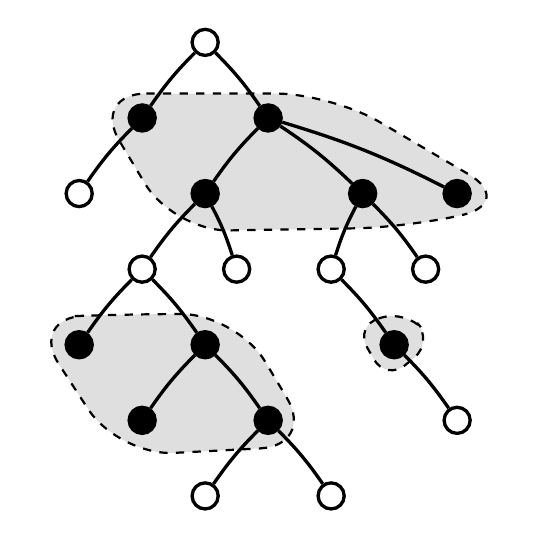
\begin{tikzpicture}[every node/.style={draw, very thick}, every path/.style={very thick}]
    
    \draw[dashed, thick, rounded corners = 20pt, fill= gray!25]
        (-1.45,5.75)  -- (1.6,5.75)-- (3.95,4.37) -- (2.6,4.05) -- (-0.4,4) -- cycle;

    \draw[dashed, thick, rounded corners = 20pt, fill= gray!25]
        (-2.24,2.9) -- (-1,2.95) -- (0.4,2.95) -- (1.4,1.28) -- (-1.1,1.15) -- cycle;

    \draw[dashed, thick, rounded corners = 9pt, fill= gray!25]
        (1.9,2.8)  -- (2.55,3)  -- (2.9,2.6) -- (2.3,2.1) -- cycle;
    
    \node[circle, draw, fill=white] (1) at (0,6.4) {};
    
    \node[circle, draw, fill=black] (2) at (-0.8,5.44) {};
    \node[circle, draw, fill=black] (3) at (0.8,5.44) {};

    \node[circle, draw, fill=white] (4) at (-1.6,4.48) {};
    \node[circle, draw, fill=black] (5) at (0,4.48) {};
    \node[circle, draw, fill=black] (6) at (2.0,4.48) {};
    \node[circle, draw, fill=black] (7) at (3.2,4.48) {};
    
    \node[circle, draw, fill=white] (8) at (-0.8,3.52) {};
    \node[circle, draw, fill=white] (9) at (0.4,3.52) {};
    \node[circle, draw, fill=white] (10) at (1.6,3.52) {};
    \node[circle, draw, fill=white] (11) at (2.8,3.52) {};
    
    \node[circle, draw, fill=black] (12) at (-1.6,2.56) {};
    \node[circle, draw, fill=black] (13) at (0,2.56) {};
    \node[circle, draw, fill=black] (14) at (2.4,2.56) {};
    
    \node[circle, draw, fill=black] (15) at (-0.8,1.6) {};
    \node[circle, draw, fill=black] (16) at (0.8,1.6) {};
    \node[circle, draw, fill=white] (17) at (3.2,1.6) {};
    
    \node[circle, draw, fill=white] (18) at (0,0.64) {};
    \node[circle, draw, fill=white] (19) at (1.6,0.64) {};
    
    \draw[bend right=5] (1) to (2);
    \draw[bend left=5] (1) to (3);
    
    \draw[bend right=5] (2) to (4);
    \draw[bend right=5] (3) to (5);
    \draw[bend left=5] (3) to (6);
    \draw[bend left=5] (3) to (7);
    
    \draw[bend right=5] (5) to (8);
    \draw[bend left=5] (5) to (9);
    \draw[bend right=5] (6) to (10);
    \draw[bend left=5] (6) to (11);
    
    \draw[bend right=5] (8) to (12);
    \draw[bend left=5] (8) to (13);
    \draw[bend left=5] (10) to (14);
    
    \draw[bend right=5] (13) to (15);
    \draw[bend left=5] (13) to (16);
    \draw[bend left=5] (14) to (17);
    
    \draw[bend right=5] (16) to (18);
    \draw[bend left=5] (16) to (19);

    \end{tikzpicture}
\end{minipage}
    \begin{minipage}[t]{0.5\textwidth}
    \centering
    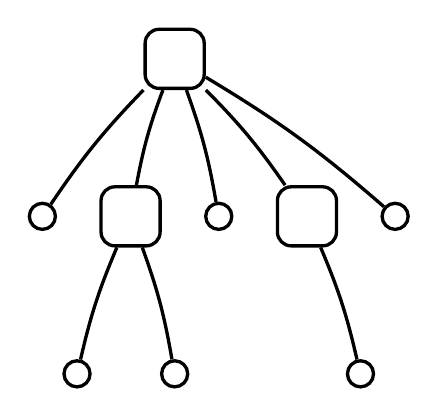
\begin{tikzpicture}[every node/.style={draw,rounded corners=5pt, very thick}, every path/.style={very thick}]
    
    \node[rectangle, minimum size=0.75cm, draw] (1) at (-0.56,10) {};
    
    \node[circle, draw] (2) at (-2.24,8) {};
    \node[rectangle, minimum size=0.75cm, draw] (3) at (-1.12,8) {};
    \node[circle, draw] (4) at (0,8) {};
    \node[rectangle, minimum size=0.75cm, draw] (5) at (1.12,8) {};
    \node[circle, draw] (6) at (2.24,8) {};
    
    \node[circle, draw] (7) at (-1.8,6) {};
    \node[circle, draw] (8) at (-0.56,6) {};
    \node[circle, draw] (9) at (1.8,6) {};
    
    \draw[bend right=5] (1) to (2);
    \draw[bend right=5] (1) to (3);
    \draw[bend left=5] (1) to (4);
    \draw[bend left=5] (1) to (5);
    \draw[bend left=5] (1) to (6);
    
    \draw[bend right=5] (3) to (7);
    \draw[bend left=5] (3) to (8);
    \draw[bend left=5] (5) to (9);

    \end{tikzpicture}
\end{minipage}
    \caption{Example of contracting 3 heavy groups. Black vertices represent heavy vertices, white vertices represent light vertices and square vertices represent light vertices with their heavy child groups contracted.}\label{exampleHeavyGroupContraction}
\end{figure}
A\textit{ heavy child group} $H_v$ is a heavy group such that $v$ is parent of some vertex $u\in H_v$. A \textit{contraction} of a heavy group $H_v$ is an operation which consists of deleting all of the vertices belonging to $H_v$ from $T$ and connecting every vertex $u$ which was a child of some vertex in $H_v$ to $v$ (for example see Figure \ref{exampleHeavyGroupContraction}). This leads to the following simple observations:

\begin{observation}
\label{monotonicityOfOptContraction}
    Let $T'$ be a tree created by contraction of a heavy group $H_v$ in $T$. Then, $\OPT\br{T'}\leq \OPT\br{T}$.
\end{observation}
\begin{observation}\label{monotonicityOfKContracion}
    Let $T'$ be a tree created by contraction of a heavy group $H_v$ in $T$. Then, $k\br{T'}\leq k\br{T}$.
\end{observation}

\subsection{Vertex ranking}\label{vertexRanking}
The vertex ranking of $T$ is a labeling of vertices $l:V\to \brc{1,2,...,\cl{\log n}}$ which satisfies the following condition: for each pair $u,v\in V\br{T}$ whenever $l(u)=l(v)$, then there exists $z\in \mathcal{P}_T\br{u,v}$ for which $l(z)>l(v)$. Such a labeling always exists and can be calculated in linear time by means of the dynamic programming \cite{Schaffer1989OptNodeRankOfTsInLinTime, Mozes_Onak2008FindOptTSStartInLinTime}. 
The vertex ranking directly induces a decision tree for $T$. The procedure is as follows:
\begin{enumerate}
    \item Let $z\in T$ be a vertex such that for every $v\in V\br{T}$: $l\br{r}\geq l\br{v}$.
    \item Schedule query to $r$ as the root of the decision tree $D$ for $T$.
    \item For each $T'\in T-r$ build a decision tree $D_{T'}$ recursively and hang every $r\br{D_{T'}}$ as a child of query to $v$ in $D$.
\end{enumerate}   

When the input tree has unitary weights the decision tree built in this way is optimal and never uses more than $\cl{\log n}$ queries.

\subsection{The main recursive procedure}\label{mainRecursiveProcedure}

We are ready to present the main recursive procedure. To avoid ambiguity, let $\mathcal{T}$ be the tree processed at some level of the recursion. Alongside $\mathcal{T}$, the algorithm takes as an input the interval $\left(a,b\right]$. For the sake of simplicity, from now on we will say that a set of vertices is a heavy group if it is a heavy group with respect to $v=\argmax_{v\in V\br{T}, w\br{v}\leq a}\brc{w(v)}$, i. e. all vertices in the heavy groups belong to $\left(a,b\right]$ and every vertex in $\left(a,b\right]$ belongs to some heavy group. The algorithm (see Algorithm \ref{createDecisionTree}) works in the following manner: 
\begin{itemize}
    \item The base case happens whenever: for every $v\in\mathcal{T}$: $w\br{v}\leq\frac{1}{\log n}$ or for every $v\in\mathcal{T}$: $w\br{v}>a$, i. e. every vertex is heavy. In such situation a solution is build by disregarding the weights of vertices and building a decision tree by using the vertex ranking of $\mathcal{T}$. 
    \item If otherwise, all heavy groups in $\mathcal{T}$ are contracted, forming a new tree $\mathcal{T}_C$ and a decision tree $D_{C}$ for $T_C$ is built in a recursive manner. By applying the following proposition, the decision tree $D$ for $\mathcal{T}$ is build by extending $D_{C}$ to contain all necessary queries in $\mathcal{T}$:
\end{itemize}
\begin{proposition}
\label{existanceOfExtensionAlgorithm}
There exists the algorithm \textsc{ExtendDecTree} which given a tree $T$, a decision tree $D_C$ for $T_C$ and an interval $\left(a,b\right]$ returns a new decision tree $D$ with cost at most:
$
\COST_{D}\br{T}\leq \COST_{D_C}\br{T_C}+\br{2+\frac{b}{a}}\cdot\OPT\br{T}
$
The algorithm runs in time 
$2^{O\br{\log^2k}}\cdot\text{poly}\br{n}$.   
\end{proposition}

The algorithm and the proof of the Proposition \ref{existanceOfExtensionAlgorithm} are provided in Section \ref{extendingTheDecisionTree}. 

\begin{algorithm}
\caption{Main recursive procedure ($n$ is a global parameter)}
\label{createDecisionTree}
\begin{algorithmic}[1]
    \Procedure{CreateDecisionTree}{$\mathcal{T}$, $\left(a,b\right]$}
        \If{$b \leq \frac{1}{\log n}$ or for every $v \in \mathcal{T}$: $ w\br{v} > a$}\Comment{\texttt{Every vertex in $\mathcal{T}$ is heavy}}
            \State \Return a decision tree $D$ built by using the vertex ranking of $\mathcal{T}$
        \Else\Comment{\texttt{There are light vertices in $\mathcal{T}$}}
            \State Create $\mathcal{T}_C$ by contracting all heavy groups in $\mathcal{T}$ 
            \State $D_C \gets$ \Call{CreateDecisionTree}{$\mathcal{T}_C$, $\left(\frac{a}{2},a\right]$} \label{recursion}
            \State $D \gets$ \Call{ExtendDecTree}{$\mathcal{T}$, $D_C$, $\left(a,b\right]$}\Comment{\texttt{Proposition \ref{existanceOfExtensionAlgorithm}}}
            \State \Return $D$
        \EndIf
    \EndProcedure
\end{algorithmic}
\end{algorithm}

\begin{lemma}\label{baseOfRecursion}
    Let $D$ be a decision tree build for $\mathcal{T}$ in the base of the recursion in \textsc{CreateDecisionTree} by using the vertex ranking of $\mathcal{T}$. Then:
$
\COST_{D}\br{\mathcal{T},w}\leq 2\OPT(T,w)
$.
\begin{proof}
    There are two cases:
    \begin{enumerate}
        \item If $b\leq \frac{1}{\log n}$ we get that:
$$
\COST_{D}\br{\mathcal{T},w}\leq\frac{\cl{\log n}}{\log n}\leq 2\leq 2\OPT(\mathcal{T},w)\leq 2\OPT(T,w)
$$

where the first inequality is due to the definition of the vertex ranking, the third inequality is due to Observation \ref{basicBoundsOnCost} and the last inequality is due to Observation
\ref{monotonicityOfOptContraction}.
\item 
If for every ${v\in \mathcal{T}} $: $w\br{v}> a$ then: For every $v\in \mathcal{T}$ let $w'\br{v}=a$ (note, that we can choose any cost here since we treat each query as unitary). As $2w'\br{v}\geq2a=b \geq w\br{v}$ we get that $2\COST_D\br{\mathcal{T}, w'}\geq \COST_D\br{\mathcal{T}, w}$. Additionally, using the fact that $w'\br{v} \leq w\br{v}$ we get that $\OPT\br{\mathcal{T}, w'}\leq \OPT\br{\mathcal{T}, w}$. Therefore:
$$
\COST_D\br{\mathcal{T}, w}\leq 2\COST_D\br{\mathcal{T}, w'}=2\OPT\br{\mathcal{T}, w'}\leq 2\OPT\br{\mathcal{T}, w}
$$

where the equality is due to the optimality of decision tree built using the vertex ranking. The lemma follows.
    \end{enumerate}
\end{proof}
\end{lemma}

We are now ready to prove the main theorem: 
\begin{theorem}
\label{parametrizedAlgorithm}
    There exists an $O\br{\log\log n}$-approximation algorithm running in time $2^{O\br{\log^2k}}\cdot\text{poly}\br{n}$.
    \begin{proof}
    Let $d$ be the depth of recursion call performed in Line $\ref{recursion}$ of the algorithm. We prove by induction that $\COST_{D}\br{\mathcal{T}, w}\leq \br{4d +2}\OPT\br{T, w}$. When $d=0$ (the base case) the induction hypothesis is true due to the Lemma \ref{baseOfRecursion}. For $d>0$ assume by induction that the cost of the decision tree build for $D_C$ is at most $\COST_{D_C}\br{\mathcal{T}_C, w}\leq \br{4(d-1) +2}\OPT\br{T, w}$. By using induction hypothesis and the fact that whenever \textsc{ExtendDecTree} is called $\frac{b}{a}\leq 2$ we get that:
    $$
    \COST_{D}\br{\mathcal{T}, w}\leq \br{4\cdot (d-1) +2}\OPT\br{T, w} + 4\OPT\br{\mathcal{T}, w} \leq \br{4d +2}\OPT\br{T, w}
    $$ 

    where the first inequality is due to the induction hypothesis and Proposition \ref{existanceOfExtensionAlgorithm} and the second inequality is due to Observation \ref{monotonicityOfOptContraction}. This proves the induction step.
    
    Let $D_T$ be a decision tree obtained by calling $\textsc{CreateDecisionTree}\br{T,\left(\frac{2^{\cl{\log\log n}-1}}{\log n},1\right]}$. As there are $\cl{\log\log\br{n}}+1$ intervals considered, the depth of recursion is bounded by $d\leq
    \cl{\log\log\br{n}}\leq \log\log\br{n}+1$. We obtain:
    $$
    \COST_{D_T}\br{T, w}
    \leq
    \br{4\log\log n + 6}\OPT\br{T, w} = O\br{\log\log n\cdot \OPT\br{T, w}}
    $$

    As $d=\text{poly}\br{n}$ and due to Observation \ref{monotonicityOfKContracion} for every $\mathcal{T}$ processed at some level of the recursion $k\br{\mathcal{T}}\leq k\br{T}$, the algorithm runs in $2^{O\br{\log^2k}}\cdot\text{poly}\br{n}$, so the theorem follows.
        
    \end{proof}
\end{theorem}
\section{Proof of Proposition \ref{existanceOfExtensionAlgorithm}: Extending the decision tree}\label{extendingTheDecisionTree}
We prove Proposition \ref{existanceOfExtensionAlgorithm} by showing the procedure $\textsc{ExtendDecTree}$ which takes as an input: the tree $T$, the partial decision tree $D_C$ for the contracted tree $T_C$ and the interval $\left(a,b\right]$ and extends $D_C$ to contain all queries needed to find any target $x\in T$. The basic idea of the algorithm is as follows: 
\begin{enumerate}
    \item Create a new decision tree used to separate heavy groups. 
    \item Build the rest of the decision tree, by using the vertex ranking to create strategy for the heavy vertices and use $D_C$ to create strategy for the light vertices. 
\end{enumerate}

To proceed, we firstly invoke the following Lemma \cite{Cicalese2016DecTreesSimEval} (under assumption that every vertex must be queried in the decision tree):
\begin{lemma}\label{subtreeCostLemma}
    Let $T'$ be a connected subtree of $T$. Then, $\OPT\br{T'}\leq\OPT\br{T}$.
\end{lemma}

We also invoke the result of \cite{dereniowski2017ApproxSsForGeneralBSinWTs} about the existence of QPTAS for the Tree Search Problem:
\begin{theorem}\label{QPTAS}
    There exists an algorithm running in $2^{O\br{\frac{\log^2n}{\epsilon^2}}}$ time, providing a $(1+\epsilon)$-approximate
solution to the Tree Search Problem for any $0 < \epsilon \leq 1$.
\end{theorem}

\subsection{The \textsc{ExtendDecTree} procedure}

\begin{algorithm}
\caption{The extension procedure}
\label{extensionProcedure}
\begin{algorithmic}[1]
    \Procedure{ExtendDecTree}{$T$, $D_C$,$\left(a,b\right]$}
        \State $\mathcal{H}\gets\brc{H\subseteq V| H \text{ is a heavy group}}$
        \State $\mathcal{X}\gets\emptyset$
        \For{$H\in\mathcal{H}$} 
        \State Pick $v\in H$ and add $v$ to $\mathcal{X}$
        \EndFor
        \State $\mathcal{Z}\gets\mathcal{Y}\gets\mathcal{X}\cup \brc{v\in T\angl{\mathcal{X}}|\deg_{T\angl{\mathcal{X}}}\br{v}\geq3}$\Comment{\texttt{Branching vertices in $T\angl{X}$.}}
        \For{$u,v\in \mathcal{Y},\mathcal{P}_{T}\br{u, v}\neq\emptyset,\mathcal{P}_{T}\br{u, v}\cap \mathcal{Y}=\emptyset$}
        \State Add $\argmin_{z\in \mathcal{P}_{T}\br{u, v}}\brc{w\br{z}}$ to $\mathcal{Z}$. \Comment{\texttt{Lightest vertex on path $P_T\br{u,v}$.}}
        \EndFor
        \State $T_{\mathcal{Z}}=\br{\mathcal{Z}, \brc{uv|\mathcal{P}_{T}\br{u, v}\cap \mathcal{Z}=\emptyset}}$
        \State $D\gets D_{\mathcal{Z}}\gets \Call{QPTAS}{T_{\mathcal{Z}}, \epsilon =1}$
        \For{$T'\in T-\mathcal{Z}$}
            \State Let $H$ be the singular heavy group in $T'$
            \State $D_{H}\gets$ a decision tree built by using the vertex ranking of $T\angl{H}$
            \State Hang $D_H$ in $D$ below the last query to a vertex $v \in N_T\br{T'}$
            \For{$L\in T'-H$}
                \State $D_L\gets $ a decision tree built by deleting all queries in $D_C$ outside of $L$
                \State Hang $D_L$ in $D$ below the last query to a vertex $v \in N_T\br{L}$
            \EndFor
        \EndFor
    \State \Return $D$
    \EndProcedure
\end{algorithmic}
\end{algorithm}
We begin with the following simple observation:
\begin{observation}
Let $\mathcal{H}$ be the set of heavy groups in $T$. Then, $\spr{\mathcal{H}}\leq k$.
\end{observation}

\begin{figure}[htp]
    \begin{minipage}[t]{0.47\textwidth}
    \centering
    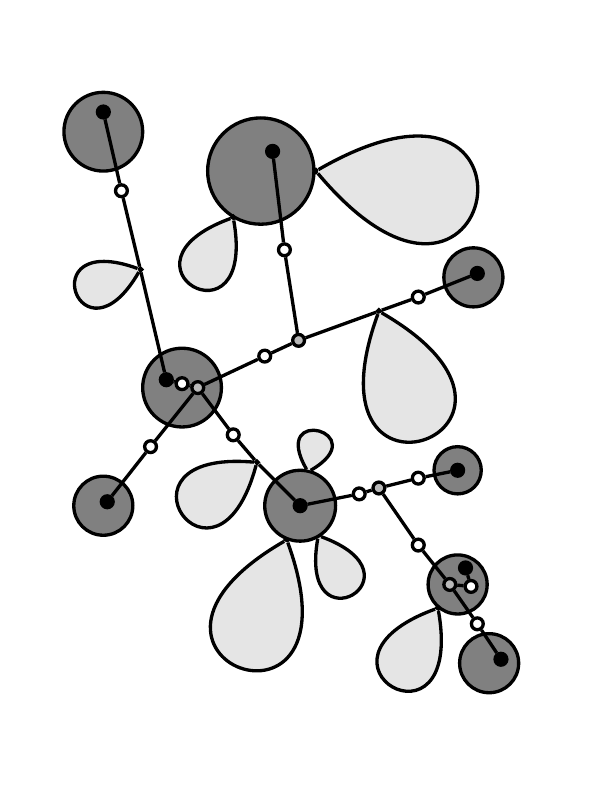
\begin{tikzpicture}[every node/.style={draw, very thick}, every path/.style={very thick}]
    
    \node[circle, draw, minimum size = 1cm, fill=gray] (1) at (-3,2.75) {};
    \node[circle, draw, minimum size=0.15cm, inner sep=0pt, fill=black] (2) at (-3,3) {};

    
    
    \node[circle, draw, minimum size = 1.35cm, fill=gray] (3) at (-1,2.25) {};
    \node[circle, draw, minimum size=0.15cm, inner sep=0pt, fill=black] (4) at (-0.85,2.5) {};
    \node[circle, draw, inner sep=0pt, fill=white] (36) at (-0.3,2.25) {};
    \node[circle, draw, inner sep=0pt, fill=white] (40) at (-1.35,1.66) {};
    

    
    \node[circle, draw, minimum size=0.15cm, inner sep=0pt, fill=white] (5) at (-2.77,2) {};
    
    \node[circle, draw, minimum size=0.15cm, inner sep=0pt, fill=white] (6) at (-0.7,1.25) {};
    
    \node[circle, draw, minimum size = 0.75cm, fill=gray] (7) at (1.7,0.9) {};
    \node[circle, draw, minimum size=0.15cm, inner sep=0pt, fill=black] (8) at (1.75,0.95) {};
    
    \node[circle, draw, inner sep=0pt, fill=white] (9) at (-2.53,1) {};
    
    \node[circle, draw, minimum size=0.15cm, inner sep=0pt, fill=white] (10) at (1,0.65) {};
    
    \node[circle, draw, inner sep=0pt, fill=white] (11) at (0.5,0.47) {};
    
    \node[circle, draw, minimum size=0.15cm, inner sep=0pt, fill=gray!55] (12) at (-0.52,0.1) {};
    
    \node[circle, draw, minimum size=0.15cm, inner sep=0pt, fill=white] (13) at (-0.95,-0.1) {};

    
    \node[circle, draw, minimum size = 1cm, fill=gray] (14) at (-2,-0.5) {};
    \node[circle, draw, minimum size=0.15cm, inner sep=0pt, fill=black] (15) at (-2.2,-0.4) {};
    \node[circle, draw, minimum size=0.15cm, inner sep=0pt, fill=white] (16) at (-2,-0.45) {};
    \node[circle, draw, minimum size=0.15cm, inner sep=0pt, fill=gray!55] (17) at (-1.8,-0.5) {};
    
    \node[circle, draw, minimum size=0.15cm, inner sep=0pt, fill=white] (18) at (-1.35,-1.1) {};

    \node[circle, draw, minimum size=0.15cm, inner sep=0pt, fill=white] (19) at (-2.4,-1.25) {};
    
    \node[circle, draw, inner sep=0pt, fill=white] (20) at (-1.05,-1.45) {};
    
    \node[circle, draw, minimum size = 0.6cm, fill=gray] (21) at (1.5,-1.55) {};
    \node[circle, draw, minimum size=0.15cm, inner sep=0pt, fill=black] (22) at (1.5,-1.55) {};
    
    \node[circle, draw, minimum size=0.15cm, inner sep=0pt, fill=white] (23) at (1,-1.65) {};
    
    \node[circle, draw, minimum size=0.15cm, inner sep=0pt, fill=gray!55] (24) at (0.5,-1.775) {};
    
    \node[circle, draw, minimum size=0.15cm, inner sep=0pt, fill=white] (25) at (0.25,-1.85) {};

    \node[circle, draw, minimum size = 0.75cm, fill=gray] (26) at (-3,-2) {};
    \node[circle, draw, minimum size=0.15cm, inner sep=0pt, fill=black] (27) at (-2.95,-1.95) {};
    \node[circle, draw, inner sep=0pt, fill=white] (41) at (-0.67,-2.433) {};
    \node[circle, draw, inner sep=0pt, fill=white] (42) at (-0.27,-2.38) {};
    \node[circle, draw, inner sep=0pt, fill=white] (43) at (-0.4,-1.57) {};
    
    \node[circle, draw, minimum size = 0.9cm, fill=gray] (28) at (-0.5,-2) {};
    \node[circle, draw, minimum size=0.15cm, inner sep=0pt, fill=black] (29) at (-0.5,-2) {};

    
    \node[circle, draw, minimum size=0.15cm, inner sep=0pt, fill=white] (30) at (1,-2.5) {};
    
    \node[circle, draw, minimum size = 0.75cm, fill=gray] (31) at (1.5,-3) {};
    \node[circle, draw, minimum size=0.15cm, inner sep=0pt, fill=gray!55] (32) at (1.4,-3) {};
    \node[circle, draw, inner sep=0pt, fill=white] (37) at (1.25,-3.3) {};
    \node[circle, draw, minimum size=0.15cm, inner sep=0pt, fill=black] (38) at (1.6,-2.79) {};
    \node[circle, draw, minimum size=0.15cm, inner sep=0pt, fill=white] (39) at (1.67,-3.025) {};
    
    \node[circle, draw, minimum size=0.15cm, inner sep=0pt, fill=white] (33) at (1.75,-3.5) {};
    
    \node[circle, draw, minimum size = 0.75cm, fill=gray] (34) at (1.9,-4) {};
    \node[circle, draw, minimum size=0.15cm, inner sep=0pt, fill=black] (35) at (2.05,-3.95) {};
    
    \draw[] (2) to (5);
    \draw[] (4) to (6);
    \draw[] (5) to (9);
    \draw[] (6) to (12);
    \draw[] (8) to (10);
    \draw[] (9) to (15);
    \draw[] (10) to (11);
    \draw[] (11) to (12);
    \draw[] (12) to (13);
    \draw[] (13) to (17);
    \draw[] (15) to (16);
    \draw[] (16) to (17);
    \draw[] (17) to (18);
    \draw[] (17) to (19);
    \draw[] (18) to (20);
    \draw[] (19) to (27);
    \draw[] (20) to (29);
    \draw[] (22) to (23);
    \draw[] (23) to (24);
    \draw[] (24) to (25);
    \draw[] (24) to (30);
    \draw[] (25) to (29);
    \draw[] (30) to (32);
    \draw[] (32) to (33);
    \draw[] (32) to (39);
    \draw[] (33) to (35);
    \draw[] (38) to (39);
    \draw[very thick, fill=gray!20]
    (9).. controls +(-120:1.5cm) and +(-200:1.5cm).. (9);
    \draw[very thick, fill=gray!20]
    (11).. controls +(-30:3cm) and +(-110:3cm).. (11);
    \draw[very thick, fill=gray!20]
    (20).. controls +(-105:2cm) and +(-185:2cm).. (20);
    \draw[very thick, fill=gray!20]
    (36).. controls +(30:3.6cm) and +(-50:3.6cm).. (36);
    \draw[very thick, fill=gray!20]
    (37).. controls +(-80:2cm) and +(-160:2cm).. (37);
    \draw[very thick, fill=gray!20]
    (40).. controls +(-80:1.75cm) and +(-160:1.75cm).. (40);
    \draw[very thick, fill=gray!20]
    (41).. controls +(-70:3cm) and +(-150:3cm).. (41);
    \draw[very thick, fill=gray!20]
    (42).. controls +(-20:1.5cm) and +(-100:1.5cm).. (42);
    \draw[very thick, fill=gray!20]
    (43).. controls +(120:1cm) and +(30:1cm).. (43);
    
    \end{tikzpicture}
    \caption{Tree $T$. Dark grey circles represent heavy groups. Light grey regions represent light subtrees. Black vertices represent $\mathcal{X}$. Gray and black vertices represent $\mathcal{Y}$. White, gray and black vertices represent $\mathcal{Z}$. Lines represent paths of vertices between vertices of $\mathcal{Z}$.}\label{exampleTreeWithSetZ}
\end{minipage}
    \hspace{0.06\textwidth} % Add space between the two minipages
    \begin{minipage}[t]{0.47\textwidth}
    \centering
    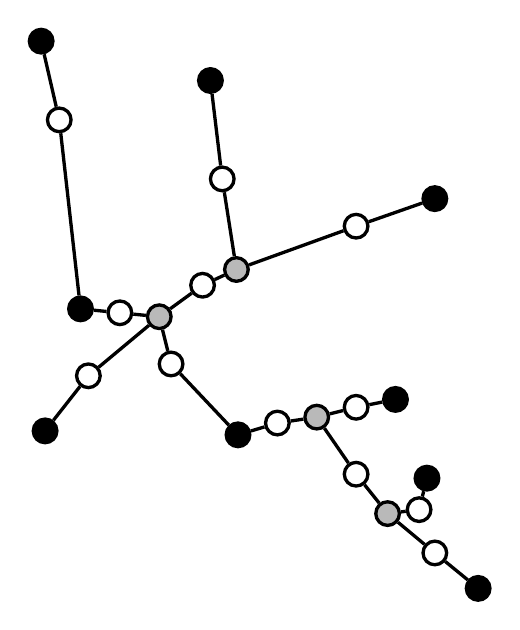
\begin{tikzpicture}[every node/.style={draw, very thick}, every path/.style={very thick}]
    
    \node[circle, draw, minimum size=0.3cm, inner sep=0pt, fill=black] (2) at (-3,4) {};

    
    
    \node[circle, draw, minimum size=0.3cm, inner sep=0pt, fill=black] (4) at (-0.85,3.5) {};
    

    
    \node[circle, draw, minimum size=0.3cm, inner sep=0pt, fill=white] (5) at (-2.77,3) {};
    
    \node[circle, draw, minimum size=0.3cm, inner sep=0pt, fill=white] (6) at (-0.7,2.25) {};
    
    \node[circle, draw, minimum size=0.3cm, inner sep=0pt, fill=black] (8) at (2,2) {};
    
    
    \node[circle, draw, minimum size=0.3cm, inner sep=0pt, fill=white] (10) at (1,1.65) {};
    
    
    \node[circle, draw, minimum size=0.3cm, inner sep=0pt, fill=gray!55] (12) at (-0.52,1.1) {};
    
    \node[circle, draw, minimum size=0.3cm, inner sep=0pt, fill=white] (13) at (-0.95,0.9) {};

    
    \node[circle, draw, minimum size=0.3cm, inner sep=0pt, fill=black] (15) at (-2.5,0.6) {};
    \node[circle, draw, minimum size=0.3cm, inner sep=0pt, fill=white] (16) at (-2,0.55) {};
    \node[circle, draw, minimum size=0.3cm, inner sep=0pt, fill=gray!55] (17) at (-1.5,0.5) {};
    
    \node[circle, draw, minimum size=0.3cm, inner sep=0pt, fill=white] (18) at (-1.35,-0.1) {};

    \node[circle, draw, minimum size=0.3cm, inner sep=0pt, fill=white] (19) at (-2.4,-0.25) {};
    
    
    \node[circle, draw, minimum size=0.3cm, inner sep=0pt, fill=black] (22) at (1.5,-0.55) {};
    
    \node[circle, draw, minimum size=0.3cm, inner sep=0pt, fill=white] (23) at (1,-0.65) {};
    
    \node[circle, draw, minimum size=0.3cm, inner sep=0pt, fill=gray!55] (24) at (0.5,-0.775) {};
    
    \node[circle, draw, minimum size=0.3cm, inner sep=0pt, fill=white] (25) at (0,-0.85) {};

    \node[circle, draw, minimum size=0.3cm, inner sep=0pt, fill=black] (27) at (-2.95,-0.95) {};
    
    \node[circle, draw, minimum size=0.3cm, inner sep=0pt, fill=black] (29) at (-0.5,-1) {};

    
    \node[circle, draw, minimum size=0.3cm, inner sep=0pt, fill=white] (30) at (1,-1.5) {};
    
    \node[circle, draw, minimum size=0.3cm, inner sep=0pt, fill=gray!55] (32) at (1.4,-2) {};
    \node[circle, draw, minimum size=0.3cm, inner sep=0pt, fill=black] (38) at (1.9,-1.55) {};
    \node[circle, draw, minimum size=0.3cm, inner sep=0pt, fill=white] (39) at (1.8,-1.95) {};
    
    \node[circle, draw, minimum size=0.3cm, inner sep=0pt, fill=white] (33) at (2,-2.5) {};
    
    \node[circle, draw, minimum size=0.3cm, inner sep=0pt, fill=black] (35) at (2.55,-2.95) {};
    
    \draw[] (2) to (5);
    \draw[] (4) to (6);
    \draw[] (5) to (15);
    \draw[] (6) to (12);
    \draw[] (8) to (10);
    \draw[] (10) to (12);
    \draw[] (12) to (13);
    \draw[] (13) to (17);
    \draw[] (15) to (16);
    \draw[] (16) to (17);
    \draw[] (17) to (18);
    \draw[] (17) to (19);
    \draw[] (18) to (29);
    \draw[] (19) to (27);
    \draw[] (22) to (23);
    \draw[] (23) to (24);
    \draw[] (24) to (25);
    \draw[] (24) to (30);
    \draw[] (25) to (29);
    \draw[] (30) to (32);
    \draw[] (32) to (33);
    \draw[] (32) to (39);
    \draw[] (33) to (35);
    \draw[] (38) to (39);
    \end{tikzpicture}
    \caption{Auxiliary tree $T_{\mathcal{Z}}$ built from vertices of set $\mathcal{Z}$. Lines represent edges between vertices of $T_{\mathcal{Z}}$.}\label{exampleAuxTreeTZ}
\end{minipage}
\end{figure}

To build a solution (see Algorithm \ref{extensionProcedure}) we will firstly define a set of vertices $\mathcal{X}$. For every $H\in\mathcal{H}$ pick arbitrary $v\in H$ and add it to $\mathcal{X}$. We also define set $\mathcal{Y}$ which consists of vertices in $\mathcal{X}$ and all vertices in $T\angl{X}$ which have degree at least 3. 

Furthermore, we define set $\mathcal{Z}$ as a set consisting of all vertices in $\mathcal{Y}$ and for every $u,v\in \mathcal{Y}$ such that $\mathcal{P}_{T}\br{u, v}\neq\emptyset$ and $\mathcal{P}_{T}\br{u, v}\cap \mathcal{Y}=\emptyset$ we add to $\mathcal{Z}$ the vertex $\argmin_{z\in \mathcal{P}_{T}\br{u, v}}\brc{w\br{z}}$ (for example see Figure \ref{exampleTreeWithSetZ}). We then create an auxiliary tree $T_{\mathcal{Z}}=\br{\mathcal{Z},\brc{uv|\mathcal{P}_{T}\br{u, v}\cap \mathcal{Z}=\emptyset}}$ (for example see Figure \ref{exampleAuxTreeTZ}). The algorithm builds a decision tree $D_{\mathcal{Z}}$ for $T_{\mathcal{Z}}$ by taking $\epsilon=1$ and applying the QPTAS from Theorem \ref{QPTAS}. Observe, that:
\begin{observation}\label{CostDZinTObservation}
    $\COST_{D_{\mathcal{Z}}}\br{T_{\mathcal{Z}}, w}=\COST_{D_{\mathcal{Z}}}\br{T, w}$.
\end{observation}

Let $D = D_{\mathcal{Z}}$. For each connected component $T'\in T-\mathcal{Z}$ we build a new decision tree in the following way: By construction of $\mathcal{Z}$, heavy vertices in $T'$ form a singular heavy group $H\subseteq V\br{T'}$. We create a new decision tree $D_H$ for $H$ by using the vertex ranking of $T\angl{H}$ and we hang $D_{H}$ in $D$ below the last query to a vertex in $N_T\br{T'}$. Then for each $L\in T'-H$ we create a decision tree $D_L$ by deleting all queries in $D_C$ to vertices outside of $V\br{L}$ and hang $D_L$ in $D$ below the last query to vertex in $N_T\br{L}$. After all these steps we obtain a valid decision tree $D$ for $T$.
\begin{lemma}\label{auxTreeSizeLemma}
    Let $T_{\mathcal{Z}}$ be the auxiliary tree. Then, $\spr{V\br{T_{\mathcal{Z}}}}\leq 4k-3$.
    \begin{proof}
        We firstly show that $\spr{\mathcal{Y}}\leq 2k-1$. We use induction on the set $\mathcal{H}$. We will construct a family of sets $\mathcal{H}_1, \mathcal{H}_2,..., \mathcal{H}_{\spr{\mathcal{H}}}$ such that for any $1\leq h\leq \spr{\mathcal{H}}$: $\spr{\mathcal{H}_h}=h$ and $\mathcal{H}_{\spr{\mathcal{H}}}=\mathcal{H}$. For each $\mathcal{H}_h$ we will also construct a corresponding set $\mathcal{Y}_h$, ensuring that in the end $\mathcal{Y}_{\spr{\mathcal{H}}}=\mathcal{Y}$.
        
        Let $\mathcal{H}_1=\emptyset$, $\mathcal{Y}_1=\emptyset$. Pick any heavy group $H\subseteq V\br{T}$ and add it to $\mathcal{H}_1$. Additionally, add the unique vertex in $H\cap\mathcal{X}$ to $\mathcal{Y}$, so that $\spr{\mathcal{Y}_1}=1$. Assume by induction on $h\geq1$ that $\spr{\mathcal{Y}_h}\leq 2h-1$. We say that heavy groups $H_1,H_2\subseteq V\br{T}$ are neighbors when for every heavy group $H_3\subseteq V\br{T}$ such that $H_3\neq H_1,H_2$: $P_T\br{H_1,H_2}\cap H_3=\emptyset$.
        Let $H\subseteq V\br{T}$ such that $H\notin \mathcal{H}_h$ be a heavy group which is a neighbor of some heavy group in $\mathcal{H}_h$. Let $\mathcal{H}_{h+1}=\mathcal{H}_h\cup\brc{H}$.  Let $z$ be the unique vertex in $H\cap\mathcal{X}$ and $\mathcal{Y}_{h+1}=\mathcal{Y}_{h}\cup\brc{z}$. Let $T_{h+1}=T\angl{\brc{v\in \mathcal{Y}_{h+1}|\mathcal{P}_T\br{v,z}\cap \mathcal{Y}_{h+1}=\emptyset}}$. Notice that $T_{h+1}$ is a spider (tree with at most one vertex with degree above 3). Add to $\mathcal{Y}_{h+1}$ the unique vertex $v\in T_{h+1}$ such that $\deg_{T_{h+1}}\br{v}\geq 3$ if it exists. Clearly, $\spr{\mathcal{Y}_{h+1}}\leq2h+1$, so the induction step is complete. By construction, eventually $\mathcal{H}_{\spr{\mathcal{H}}}=\mathcal{H}$ and $\mathcal{Y}_{\spr{\mathcal{H}}}=\mathcal{Y}$, so in consequence $\spr{\mathcal{Y}}\leq 2\spr{\mathcal{H}}-1\leq 2k-1$.
        
        As paths between vertices in $\mathcal{Y}$ form a tree, at most $2k-2$ additional vertices are added to $\mathcal{Y}$ while constructing $\mathcal{Z}$ (at most one for each path) and the lemma follows.
    \end{proof}
\end{lemma}
\begin{lemma}\label{auxTreeCostLemma}
    Let $T_{\mathcal{Z}}$ be the auxiliary tree. Then, $\OPT\br{T_{\mathcal{Z}}, w}\leq \OPT\br{T, w}$.
    \begin{proof}
        Let $D^*$ be the optimal strategy for $T\angl{\mathcal{Z}}$. We build a new decision tree $D_{\mathcal{Z}}'$ for $T_{\mathcal{Z}}$ by transforming $D^*$: Let $u,v\in \mathcal{Y}$ such that $\mathcal{P}_{T}\br{u, v}\neq\emptyset$ and $\mathcal{P}_{T}\br{u, v}\cap \mathcal{Y}=\emptyset$. Let $q\in V\br{D^*}$ such that $m\br{q}\in \mathcal{P}_{T}\br{u, v}$ be the first query among vertices of $\mathcal{P}_{T}\br{u, v}$. We replace $q$ in $D^*$ by the query to the distinct vertex $v_{u,v}\in \mathcal{P}_{T}\br{u, v}\cap \mathcal{Z}$ and delete all queries to vertices $\mathcal{P}_{T}\br{u, v}-v_{u,v}$ from $D^*$. By construction, $D_{\mathcal{Z}}'$ is a valid decision tree for $T_{\mathcal{Z}}$ and as for every $z\in \mathcal{P}_{T}\br{u, v}$: $w\br{v_{u,v}}\leq w\br{z}$ such strategy has cost at most $\COST_{D_{\mathcal{Z}}'}\br{T_{\mathcal{Z}}, w}\leq \OPT\br{T\angl{\mathcal{Z}}, w}$. We get:
        $$
        \OPT\br{T_{\mathcal{Z}}, w}\leq \COST_{D_{\mathcal{Z}}'}\br{T_{\mathcal{Z}}, w}\leq \OPT\br{T\angl{\mathcal{Z}}, w}\leq \OPT\br{T, w}
        $$

        where the first inequality is due to the optimality and the last inequality is due to the fact that $T\angl{\mathcal{Z}}$ is a subtree of $T$ (by Lemma \ref{subtreeCostLemma}). The lemma follows.
    \end{proof}
\end{lemma}
\begin{lemma}
    $\COST_D\br{T,w}\leq\COST_{D_C}\br{T_C,w}+\br{2+\frac{b}{a}}\OPT\br{T,w}$
    \begin{proof}
    We firstly show that $\COST_{D_H}\br{T\angl{H}, w}\leq \frac{b}{a}\cdot\OPT\br{T, w}$. For every $v\in H$ let $w'\br{v}=a$ (note, that we can choose any cost here since we treat each query as unitary). As $\frac{bw'\br{v}}{a}\geq b \geq w\br{v}$ we get that $\frac{b}{a}\cdot\COST_{D_H}\br{T\angl{H}, w'}\geq \COST_{D_H}\br{T\angl{H}, w}$. Additionally, using the fact that $w'\br{v} \leq w\br{v}$ we get that $\OPT\br{T\angl{H}, w'}\leq \OPT\br{T\angl{H}, w}$. Therefore:
    $$
    \begin{gathered}
        \COST_{D_H}\br{T\angl{H}, w}\leq \frac{b}{a}\cdot\COST_{D_H}\br{T\angl{H}, w'}=\frac{b}{a}\cdot\OPT\br{T\angl{H}, w'}\leq \\
        \leq
        \frac{b}{a}\cdot\OPT\br{T\angl{H}, w}\leq \frac{b}{a}\cdot\OPT\br{T, w}
    \end{gathered}
    $$
        
    where the last inequality is due to the fact that $T\angl{H}$ is a subtree of $T$ (by Lemma \ref{subtreeCostLemma}).
        
    Let $Q_D\br{T,x}$ be a sequence of queries performed in order to find target $x$. By construction of the Algorithm \ref{extensionProcedure}, $Q_D\br{T,x}$ consists of at most three distinct subsequences of queries (some subsequences might be empty). Firstly, there is a sequence of queries belonging to $Q_{D_{\mathcal{Z}}}\br{T_{\mathcal{Z}},x}$. If $x\notin \mathcal{Z}$, then it is followed by a sequence of queries belonging to $Q_{D_{H}}\br{T\angl{H},x}$ such that $H\in T'$ is a heavy group and $x\in T'$. If $x\notin H$, at last, there is a sequence of queries belonging to $Q_{D_{L}}\br{L,x}$ for $L\in T'-H$ such that $x\in L$. 
    We have:
        $$
        \begin{gathered}
        \COST_D\br{T,w}
        \leq
        \COST_{D_{\mathcal{Z}}}\br{T, w}+\max_{T'\in T-\mathcal{Z}}\brc{\COST_{D_H}\br{T\angl{H}, w}+\max_{L\in T'-H}\brc{\COST_{D_L}\br{L, w}}}
        \leq \\ \leq
        \COST_{D_{\mathcal{Z}}}\br{T_{\mathcal{Z}}, w}+\max_{T'\in T-\mathcal{Z}}\brc{\frac{b}{a}\cdot\OPT\br{T, w}+\COST_{D_C}\br{T_C, w}}
        \leq \\ \leq 
        2\OPT\br{T_{\mathcal{Z}}, w}+\frac{b}{a}\cdot\OPT\br{T, w}+ \COST_{D_C}\br{T_C, w} \leq \COST_{D_C}\br{T_C, w} + \br{2+\frac{b}{a}}\cdot\OPT\br{T, w}
        \end{gathered}
        $$
        where the first inequality is due to the construction of the returned decision tree, the second is due to Observation \ref{CostDZinTObservation} and due to the fact that $L$ is a subtree of $T_C$ (Lemma \ref{subtreeCostLemma}), the third is due is due to Theorem \ref{QPTAS} and the last is due to Lemma \ref{auxTreeCostLemma}.
        
    \end{proof}
\end{lemma}

Using Lemma \ref{auxTreeSizeLemma} we get that the QPTAS runs in time $2^{O\br{\log^2\br{4k}}}=2^{O\br{\log^2\br{k}}}$ and all other computations can be performed in polynomial time which completes the proof of the Proposition \ref{existanceOfExtensionAlgorithm}.

\section{Conclusions and future work}

We showed that approximating the Tree Search Problem within a factor of $O\br{\log\log n}$ is FPT with respect to $k$ (the heavy group sets size). Additionally, the running time is quasipolynomial in $k$, making the algorithm more applicable.

The advantage of the solution constructed in this manner is its modular form. This creates a framework for working with the problem for various classes of trees and restrictions of weight functions. The extension procedure may be schemed differently depending on the specific properties of the input. This in turn might allow for more efficiency in dealing with the problem in the real life applications and leads to the better understanding of the approximability of the problem.

The central question in this line of research is whether there exists a constant-factor approximation algorithm that, given an arbitrary tree $T$ and weight function $w$, runs in polynomial time. We believe that the approach used in the current state-of-the-art $O\br{\sqrt{\log n}}$-approximate algorithm  \cite{dereniowski2017ApproxSsForGeneralBSinWTs}, based on recursive processing of the center of the tree is unlikely to lead to further improvement of the approximation. Instead a solution with a structure similar to the one proposed in this work could potentially reduce the approximation factor to $\text{poly}\br{\log \log n}$, since the number of weight levels to be handled is at most $O\br{\log \log n}$. This observation suggests a new line of research focused on designing effective extension procedures.

On the hardness side, it remains an open question whether inapproximability bounds can be established for this problem. Currently, the only known result is the trivial nonexistence of a constant additive-factor approximation algorithm. A promising direction for future research is to derive stronger, more sophisticated inapproximability bounds.

% An also interesting question is whether there exists a polynomial-time approximation algorithm for the average-case weighted searching with approximation ratio $o\br{\log n}$. The $O\br{\log n}$ approximation algorithms exist for the generalized problem of active Bayesian learning (see, e.g., \cite{GuptasApproxAlgsForOptDTsAndAdaptTSPPs}, \cite{Cicalese2016DecTreesSimEval}), but are based on simple greedy procedures or involved reductions to variants of the TSP problem. These results, however, are much more general, and an interesting line of research is whether there exists a better solution for trees.

%%
%% Bibliography
%%

%% Please use bibtex, 

\bibliography{lipics-v2021-sample-article}

\end{document}
